\documentclass[12pt]{article}
\setlength {\marginparwidth }{2cm}
\usepackage{amsmath}
\usepackage[margin=1 in]{geometry}
\usepackage{graphicx}
\usepackage{booktabs}
\usepackage{natbib}
\usepackage{lipsum}
\usepackage[colorlinks=true, citecolor=blue]{hyperref}
\usepackage{tabularx}
\usepackage{langsci-optional}
\usepackage{langsci-gb4e}

\title{The Effect of the COVID-19 Pandemic on Influenza Vaccination Rates in the United States}
\author{Jessica Zambuto\\
Department of Statistics, University of Connecticut} 

\begin{document}
\maketitle
\section*{Abstract}
\label{sec:Abstract}
Past research has shown that the influenza vaccination has decreased the likelihood of hospitalization within patients
that test positive for COVID-19 \citep{conlon2021impact}. Thus, maintaning high influenza vaccination rates is essential \
to decreasing the severity of COVID-19 cases. The goal of this study is to determine how influenza vaccination rates within the
United States have changed due to the pandemic by comparing proportions of those vaccinated before the pandemic, defined as 2018-2019
to those during the pandemic, defined as 2020-2021, and comparing during the pandemic to proportions after the pandemic defined as 2021-2022. 
In order to account for possible factors that influence influenza vaccination coverage, the analysis was performed on three groups: by age,
race, and the general population. Results showed that there is statistically significant evidence in favor of a difference in proportions before,
and after the COVID-19 pandemic for the various age groups and the general population. There is no statistically significant evidence of a difference
in proporitions for the racial groups.

\section*{Keywords}
\label{sec:Keywords}
Influenza Vaccine, Vaccine Hesitancy, COVID-19, Two Sample Z-Test

\section{Introduction}
\label{sec:Introduction}

\section{Data}
\label{sec:data}
Data was collected from the Centers for Disease Control and Prevention website. The CDC analyzes data yearly from two telephone surveys, 
"the National Immunization Survey-Flu (NIS-Flu) and the Behavioral Risk Factor Surveillance System (BRFSS), to estimate flu vaccination 
coverage for the U.S. population during the flu season. The NIS-Flu is a national random-digit-dialed cellular telephone survey of households.
The BRFSS is a state-based random-digit-dialed cellular and landline telephone survey which collects information on a variety of health conditions 
and risk behaviors from one randomly selected adult greater than 18 years in a household. The BRFSS includes survey questions asking whether the respondent had 
received a flu vaccination in the past 12 months, and if so, in which month and year. Responses to the flu vaccination status questions were not verified by medical records. 
Respondents who did not have either a yes or no response to the flu vaccination status question were excluded from the analysis.Flu vaccination coverage estimates from both surveys 
were calculated using Kaplan-Meier survival analysis using month of reported flu vaccination to determine cumulative flu vaccination coverage." \citep{cdc_2021}. \par
The data collected included age, region, season, vaccination type, and race/ethnicity. However, this study was only interested in the seasonal influenza vaccination, the United States,
years 2019-2020, 2020-2021, and 2021-2022, the age groups defined as $\ge6$ months, 6 months-17 years, 18-49 years, 50-64 years, and $\ge 65$ years of age, and the racial groups defined
as white, black, hispanic, and other.\par
The proporitions of those vaccinated corresponding to the variables of interest were extracted from the dataset on the CDC website and recorded in the tables below. These propotions are important
because they allowed for the two sample z test analysis to determine if the vaccination rates differed over time among these groups.\par

\begin{table}[h!]
    \centering
    \caption{Influenza Vaccination Rates by Year in the United States}
    \label{tab:table:proporitonsyear}
     \begin{tabularx}{.8\textwidth}{X rrr}
      \lsptoprule
                & 2019-2020 & 2020-2021  & 2021-2022\\
      \midrule
      Proportion  &   .518  &    .521  &    .514\\
      \lspbottomrule
     \end{tabularx}
    \end{table}

\begin{table}[h!]
    \centering
    \caption{Influenza Vaccination Rates by Year and Race in the United States}
    \label{tab:table:proporitonsrace}
     \begin{tabularx}{.8\textwidth}{X rrr}
      \lsptoprule
                & 2019-2020 & 2020-2021  & 2021-2022\\
      \midrule
      White  &   .548  &    .564  &    .546\\
      Black  &   .456  &    .427  &    .514\\
      Hispanic  &   .466  &    .449  &   .45\\
      Other  &   .518  &    .521  &    .525\\
      \lspbottomrule
     \end{tabularx}
    \end{table}

\begin{table}[h!]
    \centering
    \caption{Influenza Vaccination Rates by Year and Age in the United States}
    \label{tab:table:proporitonsage}
     \begin{tabularx}{.8\textwidth}{X rrr}
      \lsptoprule
                & 2019-2020 & 2020-2021  & 2021-2022\\
      \midrule
      $\ge6$ Months-17 years  &   .637  &    .586  &    .578\\
      18-49 years  &   .384  &    .377  &    .371\\
      50-64 years &   .506  &    .542  &    .524\\
      $\ge 65$ years  &   .698  &    .752 &   .739\\
      \lspbottomrule
     \end{tabularx}
    \end{table}

\begin{figure}[ht!]
  \centering
  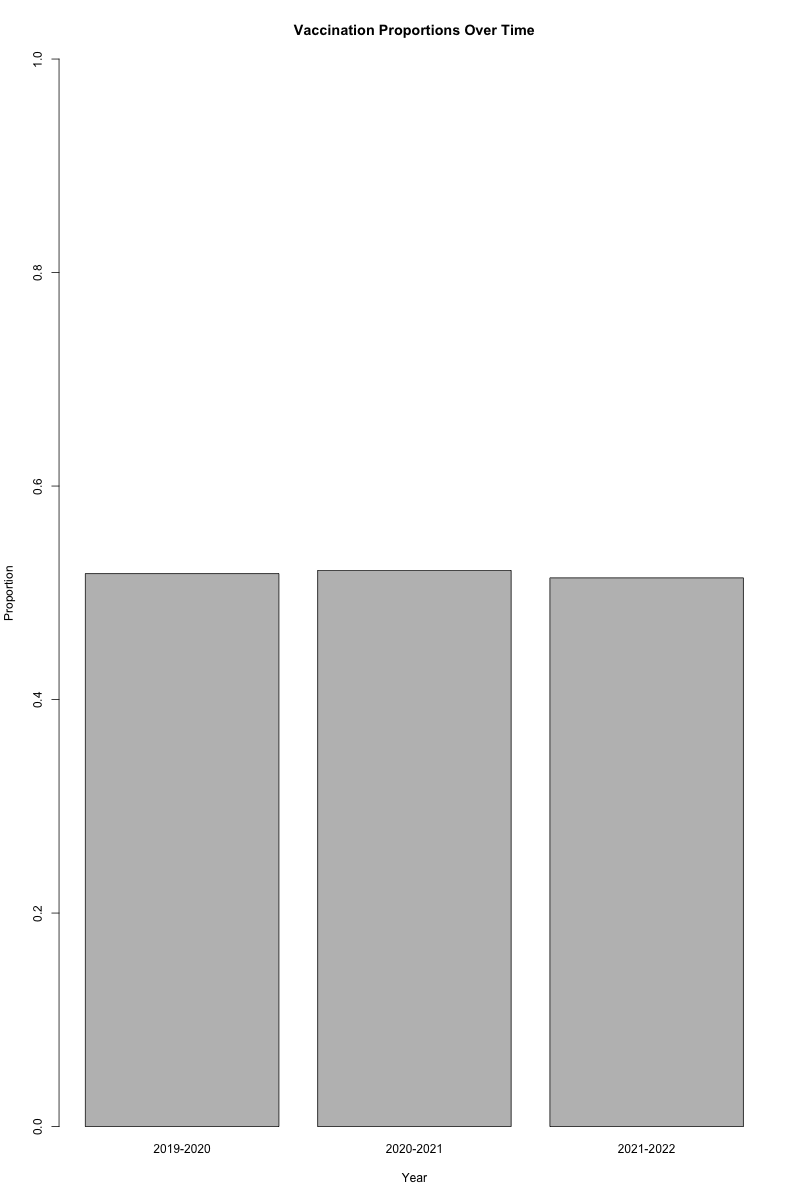
\includegraphics[width= 125mm ,scale=.5]{plot.png}
  \caption{Influenza Vaccination Proportions of Those $\ge 6$ Months Old From 2019-2022.}
  \label{fig:years}
\end{figure}

\begin{figure}[ht!]
  \centering
  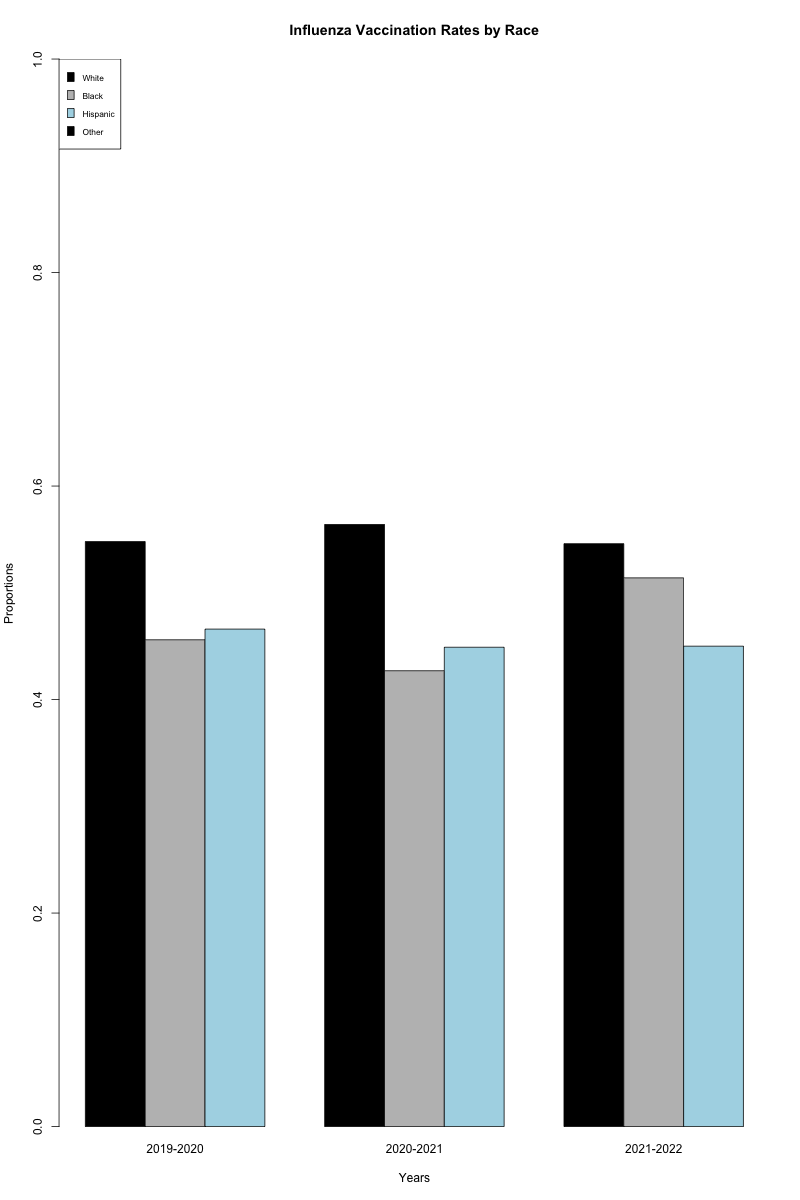
\includegraphics[width= 125mm ,scale=.75]{race.png}
  \caption{Influenza Vaccination Proportions by Race in 2019-2022.}
  \label{fig:race}
\end{figure}

\begin{figure}[ht!]
  \centering
  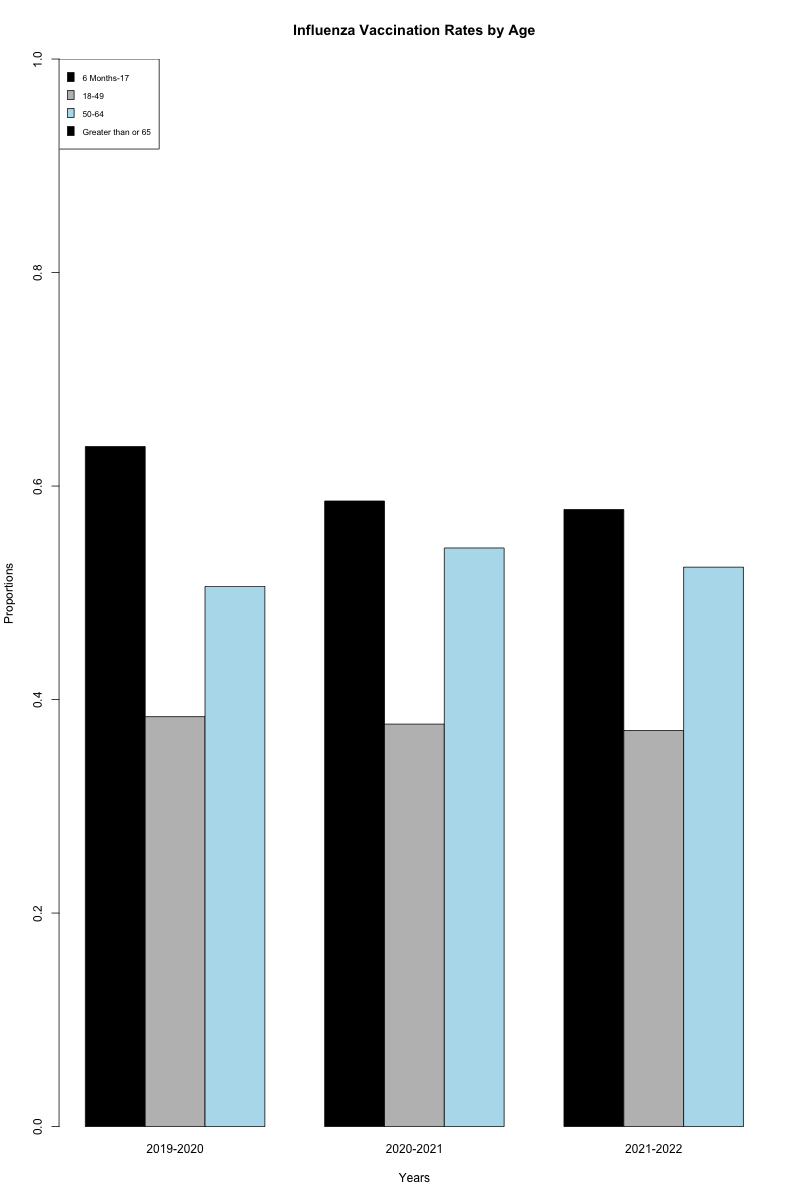
\includegraphics[width= 125mm ,scale=.5]{age.png}
  \caption{Influenza Vaccination Proportions by Age in 2019-2022.}
  \label{fig:age}
\end{figure}

\clearpage
\section{Methods}
\label{sec:Methods}

\section{Results}
\label{sec:Results}

\section{Discussion}
\label{sec:Discussion}

\clearpage
\bibliographystyle{chicago}
\bibliography{cite}
\end{document} 